\documentclass[xcolor=dvipsnames]{beamer}
\usepackage[outline]{contour}
\usepackage{transparent}
\usepackage{pgfplots}
\usepackage[utf8]{inputenc}
\usepackage{multimedia}
\usepackage{graphicx}
\usetheme{Madrid}
\usepackage{amsmath,amssymb}
\usepackage{bm}
\usepackage[absolute,overlay]{textpos}
\usepackage{mathtools}
\usepackage{courier}
\usepackage{tikz}
\tikzstyle{every picture}+=[remember picture]
\usetikzlibrary{positioning}
\usepackage{caption}
\usepackage{lmodern}
\beamertemplatenavigationsymbolsempty
\usefonttheme[onlymath]{serif}
\graphicspath{{./gfx/}}
\newcommand{\ppos}{q}
\newcommand{\pvel}{u}
\newcommand{\fpos}{r}
\newcommand{\fvel}{v}
\newcommand{\corr}{\text{corr}}
\newcommand{\dpr}{\text{\tiny DP}}
\newcommand{\qtd}{\text{\tiny q2D}}
\renewcommand{\vec}[1]{\bm{#1}}
\newcommand{\tens}[1]{\bm{\mathcal{#1}}}
\newcommand{\oper}[1]{\mathcal{#1}}
\newcommand{\uammd}{\gls{UAMMD}\xspace}
\newcommand{\gpu}{\gls{GPU}\xspace}
\newcommand{\dt}{\delta t}
\newcommand{\kT}{k_B T}
\newcommand{\sinc}{\textrm{sinc}}
\newcommand{\floor}{\textrm{floor}}
\newcommand{\near}{\textrm{near}}
\newcommand{\far}{\textrm{far}}
\newcommand{\half}{\frac{1}{2}}
\newcommand{\red}[1]{{\color{red}#1}}
\newcommand{\fou}[1]{\widehat{#1}}
\newcommand{\noise}{\widetilde{W}}

\newcommand{\executeiffilenewer}[3]{
  \ifnum
  \pdfstrcmp{\pdffilemoddate{#1}}{\pdffilemoddate{#2}}>0
  {\immediate\write18{#3}}
  \fi
}
\newcommand{\includesvg}[2][width=\columnwidth]{
  \executeiffilenewer{#2.svg}{#2.pdf}
  {inkscape -D #2.svg --export-type=pdf } %  --export-latex}
  %\def\svgwidth{#2}
  % \input{#1.pdf_tex}
  \includegraphics[#1]{#2.pdf}
}

\usepackage[absolute,overlay]{textpos}

\def\ucpp{uammd_cpp_lexer.py:UAMMDCppLexer -x}
\usepackage{tcolorbox}
\usepackage{xparse}
\tcbuselibrary{breakable,minted,xparse,skins,listings}
\usemintedstyle{default}
\setminted[\ucpp]{ %
  linenos=false,             % Line numbers
  autogobble=true,          % Automatically remove common white space
  fontsize=\small,
  breaklines
}
\AtBeginDocument{
  \newtcblisting{code2}[2][]{
    colback=white,
    colbacktitle=white,
    coltitle=black,
    pad at break*=0mm,
    listing only,
    listing engine=minted,
    listing remove caption=true,
    title={~#1},
    minted language=\ucpp,
    enhanced jigsaw,
    minipage boxed title,
    attach boxed title to bottom center={xshift=0mm,yshift=-1mm},
    boxed title style={size=small, blanker},
    center title,
    #2
  }
}
\tcbsetforeverylayer{autoparskip}


\makeatother
\setbeamertemplate{footline}
{
  \leavevmode%
  \hbox{%
  \begin{beamercolorbox}[wd=.4\paperwidth,ht=2.25ex,dp=1ex,center]{author in head/foot}%
    \usebeamerfont{author in head/foot}\insertshortauthor
  \end{beamercolorbox}%
  \begin{beamercolorbox}[wd=.6\paperwidth,ht=2.25ex,dp=1ex,center]{title in head/foot}%
    \usebeamerfont{title in head/foot}\insertshorttitle\hspace*{3em}
    \insertframenumber{} / \inserttotalframenumber\hspace*{1ex}
  \end{beamercolorbox}}%
  \vskip0pt%
}
\makeatletter
\makeatletter
\newcommand{\howmany}[2][subsection]{%
  \begingroup
  \@namedef{the#1}{\arabic{#1}}%
  \addtocounter{#1}{\m@ne}%
  \refstepcounter{#1}%
  \label{#2}%
  \endgroup}
\makeatother

\title{Complex fluids in the GPU era}
\subtitle{Algorithms and simulations}
\author{Raul P. Pelaez}

\institute{Universidad Autónoma de Madrid}
\date{\today}

%\captionsetup[figure]{font=small,skip=0pt}
\usepackage[export]{adjustbox}
\setbeamertemplate{itemize subitem}{$\rightarrow$}
\newcounter{framesectioncounter}
\AddToHook{cmd/section/before}{\setcounter{framesectioncounter}{0}}
\pdfmapfile{-mpfonts.map}
\usepackage{lmodern}
\everymath{\displaystyle}
\begin{document}


\begin{frame}
  \titlepage
  \centering
\small  Supervisor: Rafael Delgado-Buscalioni
  \begin{figure}
    \centering
    
\includegraphics[width=0.25\linewidth]{UAMlogo}
  \end{figure}
\end{frame}

%\section{This thesis main contributions}


\begin{frame}
  \frametitle{Talk outline}
  \tableofcontents[
  sectionstyle=show/show,
  subsectionstyle=hide/hide/hide,
  subsubsectionstyle=hide/hide/hide/hide
  ]
\end{frame}



%\begin{frame}
%  \frametitle{Outline}
%  \begin{itemize}
%  \item UAMMD's functionalities
%  \item Particle-based and grid based
%  \item Code structure
%    \begin{itemize}
%    \item open-source
%    \item adaptable
%    \item ...
%    \end{itemize}
%  \end{itemize}
%\end{frame}
%

\section{Introduction}
\begin{frame}
  \frametitle{Talk outline}
  \tableofcontents[
  sectionstyle=show/shaded,
  subsectionstyle=show/show/hide,
  subsubsectionstyle=show/show/show/hide
  ]
\end{frame}

\subsection{Complex fluids}
\begin{frame}
  \frametitle{Complex fluids}
\centering \Large  The coexistence between a liquid and solid phase
  \begin{figure}
    \centering
    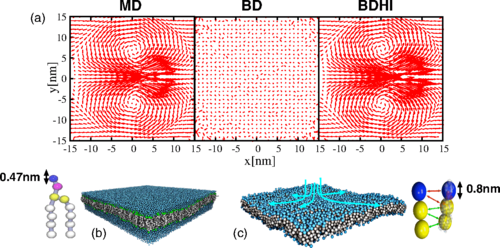
\includegraphics[width=0.5\linewidth]{membrane}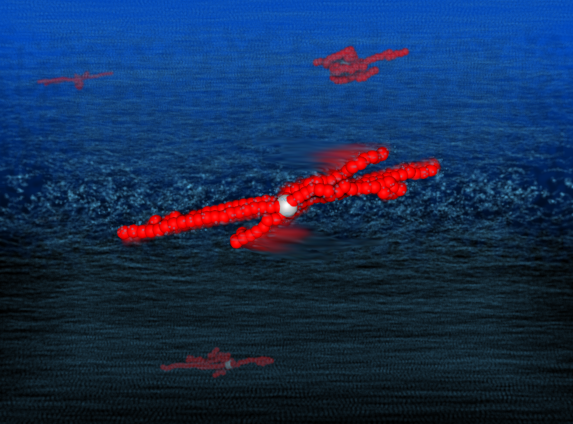
\includegraphics[width=0.2\linewidth]{star}
    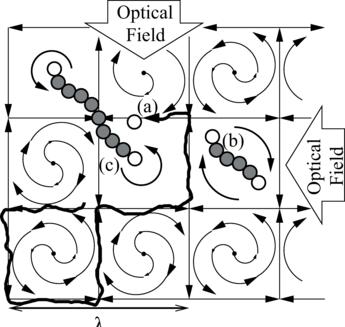
\includegraphics[width=0.2\linewidth]{optofluidics}\\
    {\fontsize{4.5}{12} \selectfont [{\bf Panzuela, S. and Delgado-Buscalioni, R.} PRL 2018.]  -  [{\bf Raul P. Pelaez and Delgado-Buscalioni, R.} Macromolecules 2020]    -   [{\bf  Mel\'endez, M.} et. al. PRE 2019.]}\\
    \only<1>{\movie[autostart,loop,poster,showcontrols=true,width=0.3\linewidth]{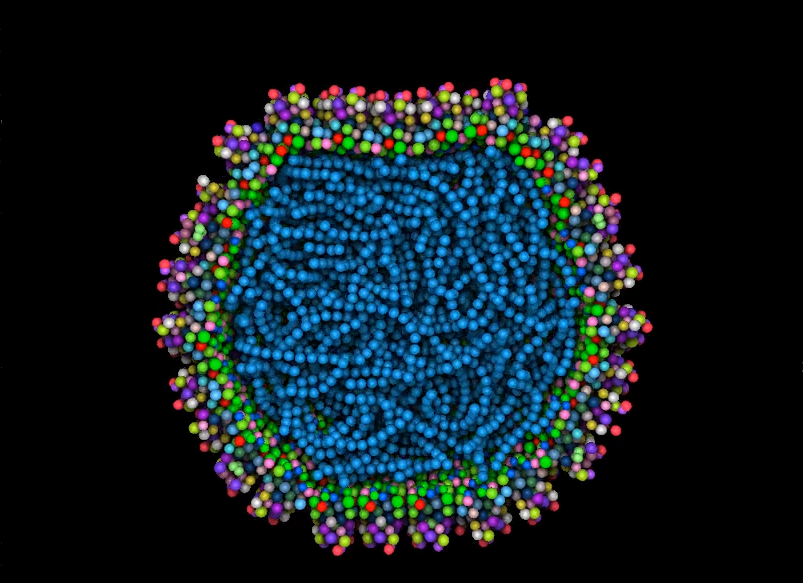
\includegraphics[width=0.3\linewidth]{virus_scr.png}}{gfx/virus.mp4}}%
    \only<2>{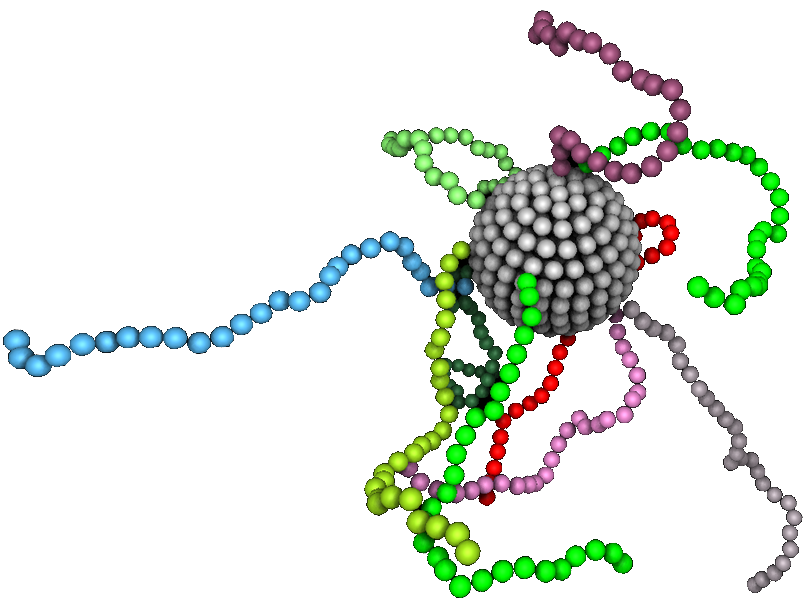
\includegraphics[width=0.235\linewidth]{lipostrandspablo.png}}%
    \movie[autostart,loop,poster,showcontrols=true,width=0.3\linewidth]{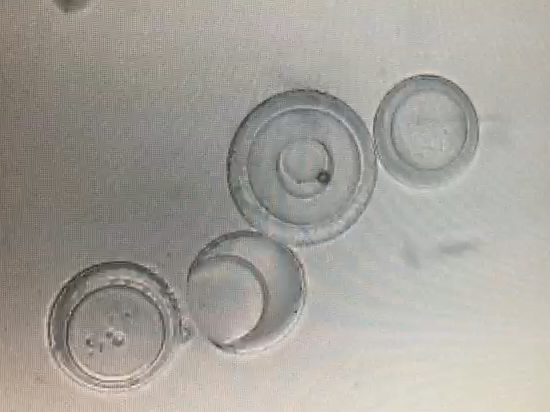
\includegraphics[width=0.3\linewidth]{rots.png}}{gfx/rots.mp4}%
    \only<1>{%
      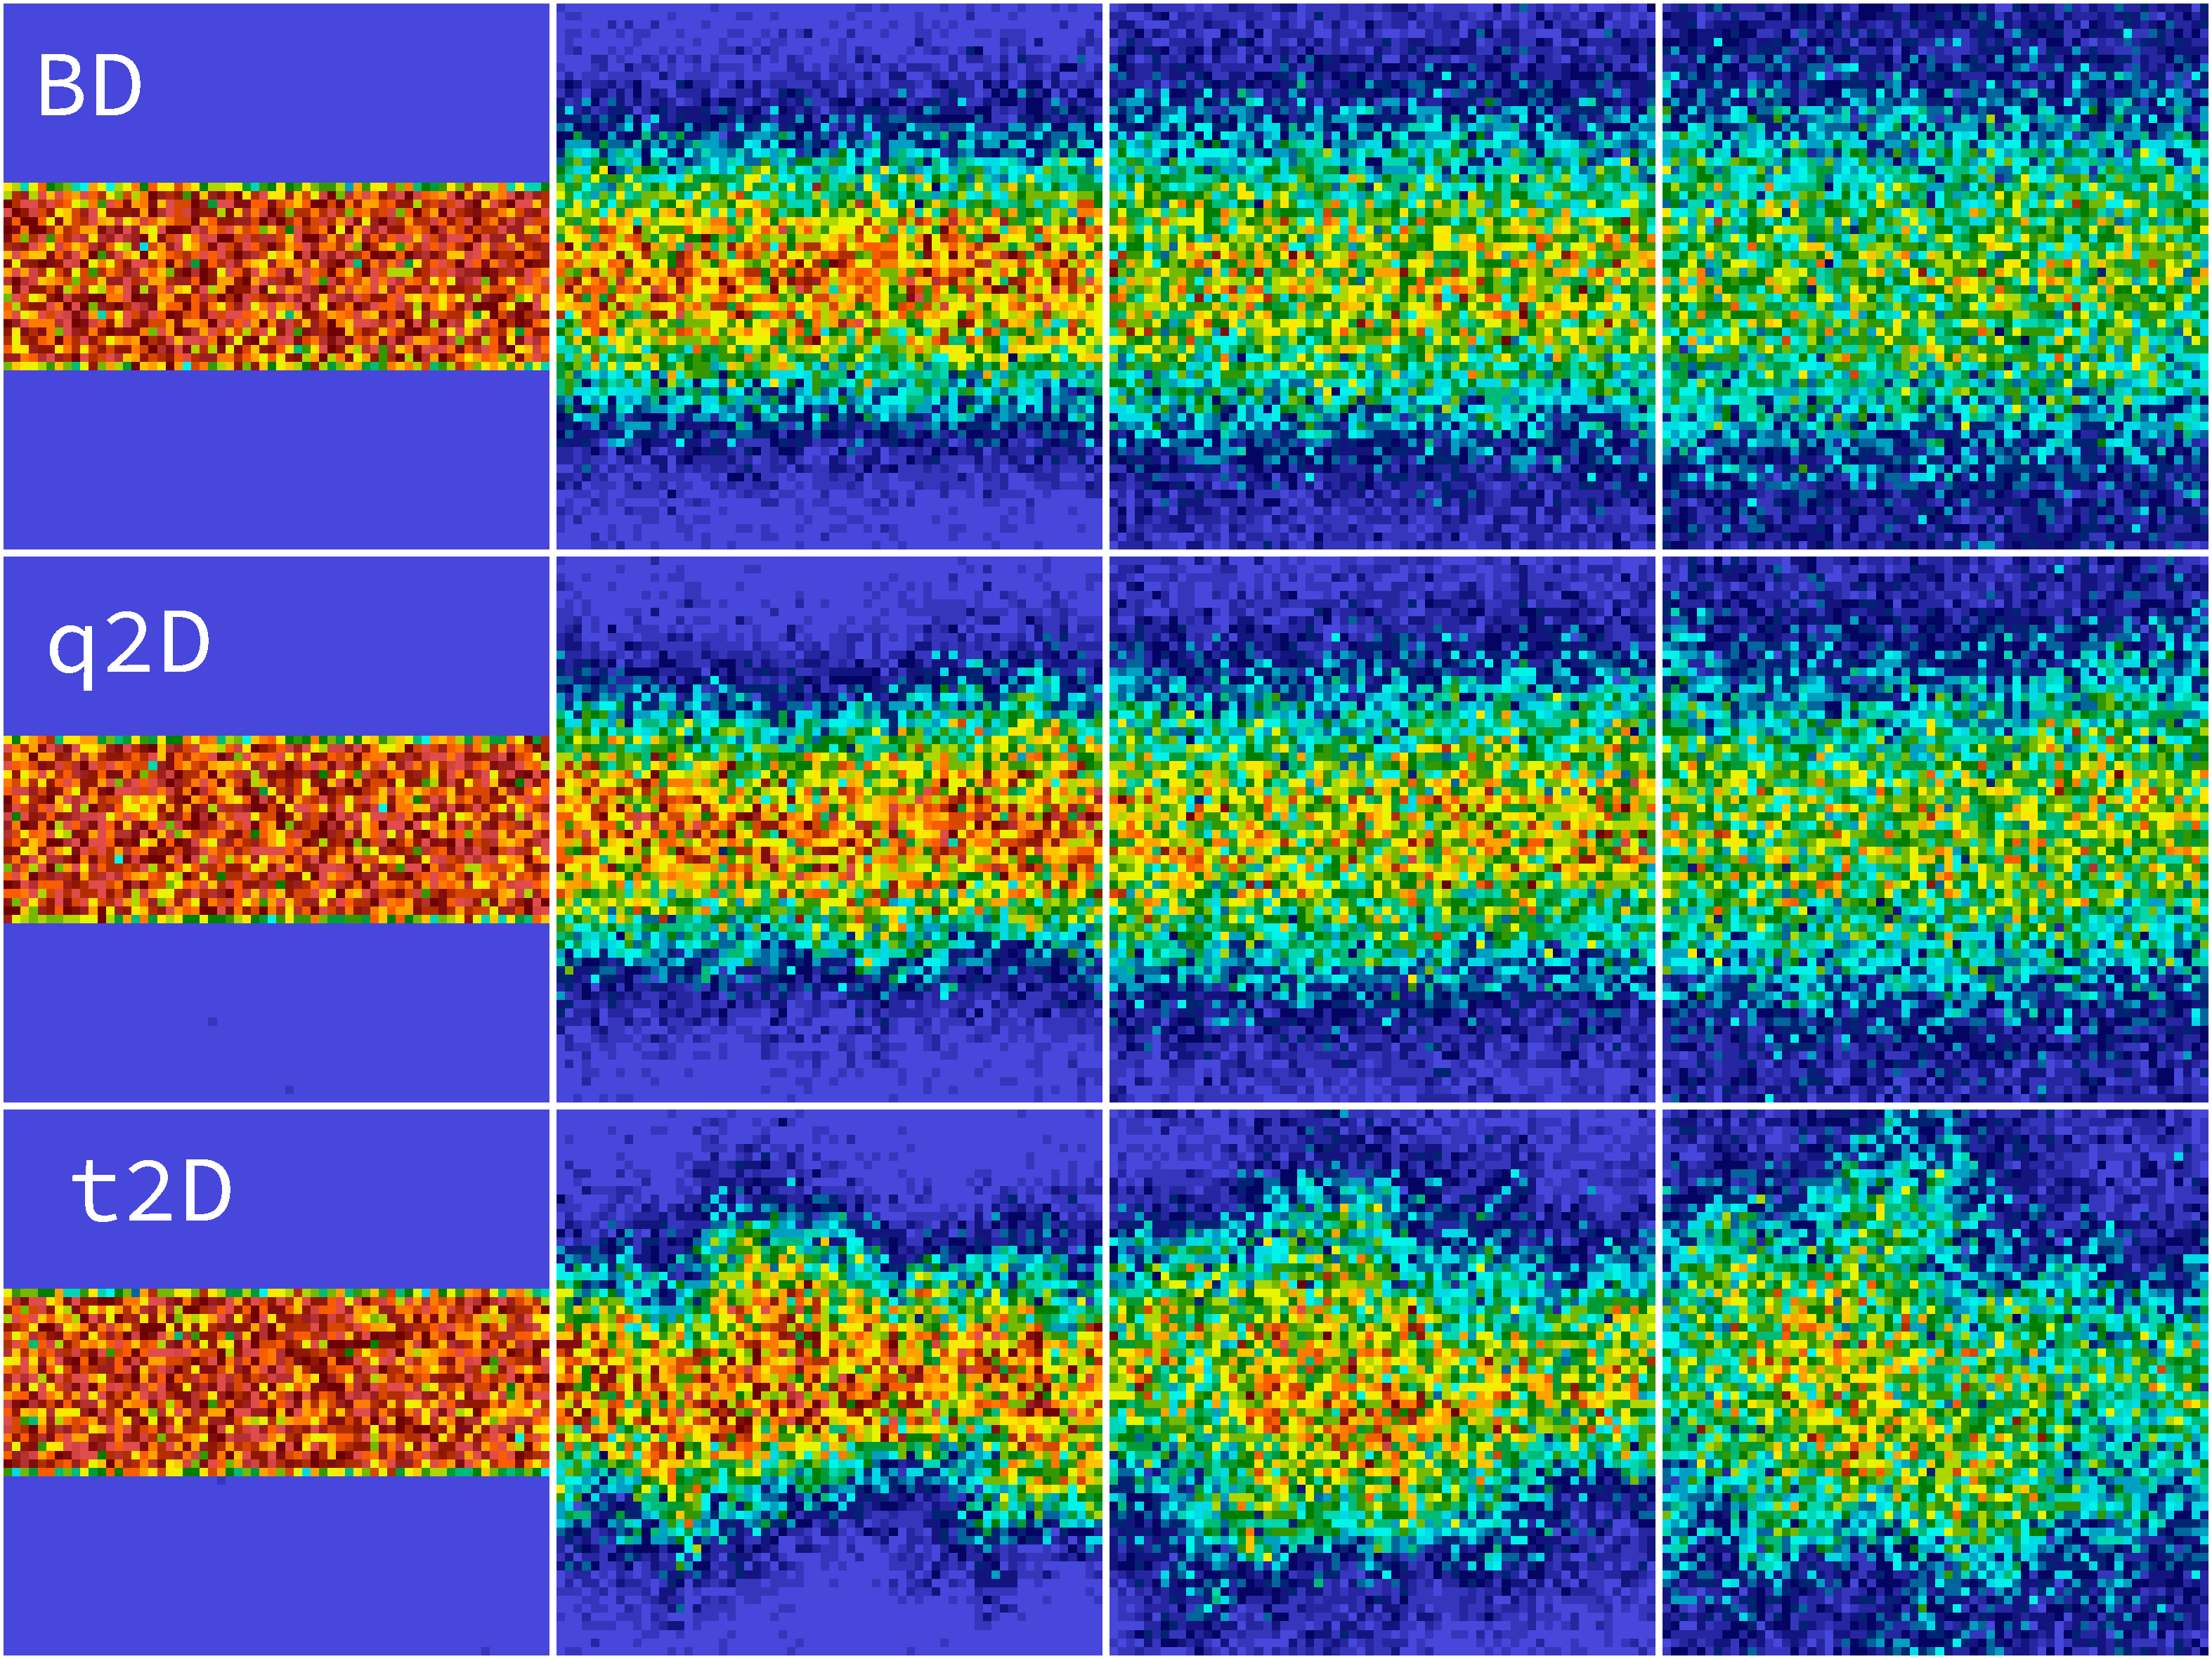
\includegraphics[width=0.3\linewidth]{q2Dcolorstripe}\\
      {\fontsize{4.5}{12} \selectfont [Courtesy of Pablo Ibañez] ------------ [Courtesy of Berta Tinao] -------------- [{\bf Raul P. Pelaez} et. al. JSTAT 2018.]}%
    }
    \only<2>{%
      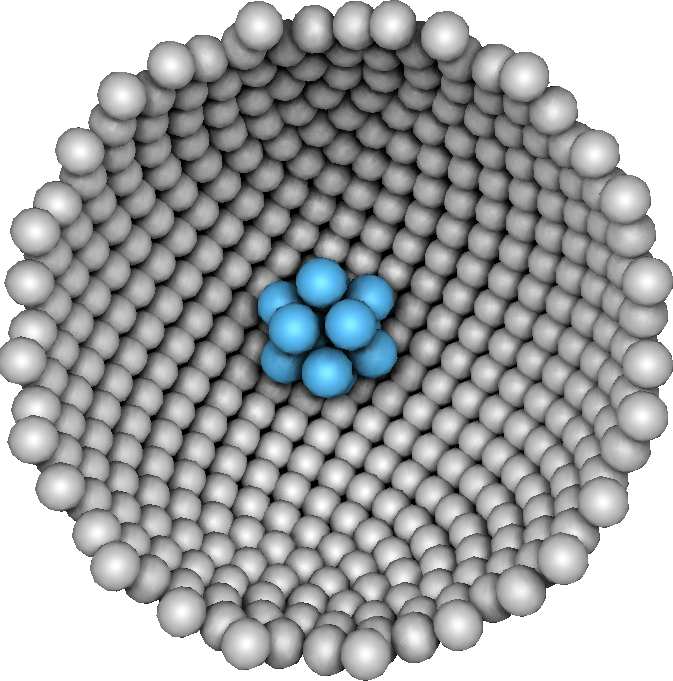
\includegraphics[width=0.22\linewidth]{mnppablo.png}\\
      {\fontsize{4.5}{12} \selectfont [Courtesy of Pablo Palacios] ------------------------ [Courtesy of Berta Tinao] ----------------------------------------- [Courtesy of Pablo Palacios]}
    }
  \end{figure}
\end{frame}


\subsubsection{Numerical techniques}
\begin{frame}
  \frametitle{Complex fluids}
  \framesubtitle{The spatio-temporal landscape of numerical techniques.}
  \begin{figure}
    \centering
    \begin{tikzpicture}
      \node[anchor=south west, inner sep=0] (image) {\includesvg[width=0.8\linewidth]{gfx/landscape}};
      \begin{scope}[shift={(image.south west)},x={(image.south east)},y={(image.north west)}]
        %\draw foreach \xy in {0,0.1,...,1.001}{(\xy,0) -- node[pos=0,below]{\pgfmathprintnumber{\xy}} (\xy,1)(0,\xy) -- node[pos=0,left]{\pgfmathprintnumber{\xy}} (1,\xy)};
        \only<2>{\filldraw[red, opacity=0.6] (0.12,1) rectangle (0.5,0.07) node[midway] (A) {};\node[above=50pt of A, black]{\contourlength{1pt}\contour{white}{\textbf{Fully Lagrangian}}};}
        \only<4>{\filldraw[blue, opacity=0.6] (0.5,1) rectangle (0.72,0.07) node[midway] (A) {};\node[below=40pt of A, black, align=left]{\contourlength{1pt}\contour{white}{\textbf{Eulerian}}\\\contourlength{1pt}\contour{white}{\textbf{Lagrangian}}};}
        \only<3>{\filldraw[green, opacity=0.6] (0.72,1) rectangle (1,0.07) node[midway] (A) {};\node[above=50pt of A, black]{\contourlength{1pt}\contour{white}{\textbf{Fully Eulerian}}};}
      \end{scope}
    \end{tikzpicture}
    \caption{Figure courtesy of Rafael Delgado-Buscalioni.}
  \end{figure}  
\end{frame}

\subsubsection{Coarse-grained levels of description}
\begin{frame}
  \frametitle{Complex fluids}
  \framesubtitle{Usual levels of coarse-grained description}
  \begin{figure}
    \centering
    \includesvg[width=0.55\linewidth]{gfx/multiscale}
  \end{figure}  
\end{frame}
\begin{frame}[t]
  \frametitle{Complex fluids}
  \framesubtitle{Usual levels of coarse-grained description}
  \begin{columns}[T]
    \begin{column}{0.5\linewidth}
        \begin{tikzpicture}
          \node[anchor = south west, inner sep = 0] (image) {\includesvg[width=\linewidth]{gfx/multiscale}};
          \begin{scope}[shift={(image.south west)},x={(image.south east)},y={(image.north west)}]
            %Draw a overlaying grid to easily see where the rectangles must be, this can be commented out in the final version
%            \draw foreach \xy in {0,0.1,...,1.001}{
%            (\xy,0) -- node[pos=0,below]{\pgfmathprintnumber{\xy}} (\xy,1)
%            (0,\xy) -- node[pos=0,left]{\pgfmathprintnumber{\xy}} (1,\xy)};
            \foreach[count=\i] \mypath in {
              {(0,1) rectangle (0.48,0.55)},
              {(0.48,1) rectangle (1.0,0.55)},
              {(0,0.55) rectangle (0.48,0)},
              {(0.48,0.55) rectangle (1,0)},
              {(0,1) rectangle (1,0)},
              {(0,1) rectangle (1,0)}
            }{
              \filldraw<\i>[white,opacity=0.9,even odd rule] (0,0) rectangle (1,1) \mypath;
            }
          \end{scope}
        \end{tikzpicture}
      \end{column}
      \begin{column}{0.45\linewidth}
      \begin{center}
        \textbf{Relevant variables:}
      \end{center}
      \begin{itemize}
      \item<1-> $\vec{q}_i$: Position of particle $i$.
      \item<1-3,5-> $\vec{u}_i$: Velocity of particle $i$.
      \item<3,5-> $\xi(\vec{q}_{ij})$: Friction kernel.
      \item<2,5-> $\vec{v}(\vec{r},t)$: Fluid velocity field.
      \item<4-> $M(\vec{q}_{ij})$: Mobility tensor.
      \end{itemize}
      \centering      
      \only<1-4>{\textbf{Tipical timescale:}\newline}
      \only<1>{$\tau \sim 10^{-12}s$}
      \only<2>{$\tau \sim 10^{-\{9-6\}}s$}
      \only<3>{$\tau \sim 10^{-5}s$}
      \only<4>{$\tau \sim 10^{-3}s$}
      \only<5->{\textbf{Timescale range:}\newline $\tau \sim [10^{-12}, 10^{-3}]s$}
    \end{column}
  \end{columns}
  \only<1>{\begin{textblock*}{0.5\linewidth}(0.05\linewidth, 0.55\paperheight)}
  \only<2>{\begin{textblock*}{0.53\linewidth}(0.05\linewidth, 0.49\paperheight)}
  \only<3>{\begin{textblock*}{0.5\linewidth}(0.05\linewidth, 0.2\paperheight)}
  \only<4,5>{\begin{textblock*}{0.5\linewidth}(0.05\linewidth, 0.17\paperheight)}
  \only<6>{\begin{textblock*}{0.99\linewidth}(0.04\linewidth,0.23\paperheight)}
    \begin{block}<1-4>{
        \only<1>{Molecular Dynamics (MD)}
        \only<2>{Immersed Boundary Method (IBM)}
        \only<3>{Langevin Dynamics (LD)}
        \only<4>{Brownian Dynamics (BD)}
      }{$$\only<1>{%
          \begin{aligned}
            m\ddot{\vec{\ppos}} &= \vec{F}\\
            \vec{\pvel} &= \dot{\vec{\ppos}}
          \end{aligned}
        }%
      \only<2>{%
          \begin{aligned}
            &\rho\partial_t\vec{\fvel} = -\vec{\partial}_{\vec{\fpos}}\cdot \tens{\sigma} + \vec{f} + \text{fluct}\\
            \int_{V_p}\vec{f}d\vec{\fpos} &= \vec{F}_i\quad\text{and}\quad \vec{u}_i = \int_{V_p}\vec{\fvel}d\vec{\fpos}
          \end{aligned}%
       }%
      \only<3>{m d\vec{\pvel} = \vec{F}dt - \xi\vec{\pvel}dt +  \sqrt{2\xi\kT}\vec{\noise}}%
      \only<4>{%
          \begin{aligned}%
            d\vec{\ppos} =& \tens{M}\vec{F}dt + \sqrt{2\kT\tens{M}}d\vec{\noise}\\%
                          &+ \kT\vec{\partial}_{\vec{\ppos}}\cdot\tens{M}dt.%
          \end{aligned}%
        }%
        $$}
    \end{block}
    \begin{alertblock}<6>{\centering \Large We always have}
      \centering \Large
      Interacting \emph{particles} with a \emph{state} that \emph{evolves}.
    \end{alertblock}
  \end{textblock*}
  \centering
  \only<1>{
    Supervector notation $\vec{q} := \{\vec{q}_1,\dots,\vec{q}_N\}$
  }
  \only<2>{
    $\partial_t := \frac{\partial}{\partial t} \rightarrow \vec{\partial}_{\vec{r}} := \nabla := \left(\partial_x,\partial_y,\partial_z\right) $ 
  }
  \only<3>{
    $\vec{\noise}$: Wienner increments, $\mathcal{N}(0,dt)$
  }
  \only<4>{
    $d\vec{\noise}$: Wienner increments, $\mathcal{N}(0,dt)$
  }
\end{frame}

\section{Building blocks of a complex fluid simulation algorithm}
\begin{frame}
  \frametitle{Talk outline}
  \tableofcontents[
  sectionstyle=show/shaded,
  subsectionstyle=show/show/hide,
  subsubsectionstyle=show/show/show/hide
  ]
\end{frame}


% \subsection{Computational Challenges}



\begin{frame}
  \frametitle{Computational challenges in soft matter simulation}
  \setbeamercovered{transparent=40}
  \begin{columns}[T]
    \begin{column}{0.6\linewidth}
      \begin{enumerate}
        \Large
      \item Short range interactions
      \item<1> Long range interactions
      \item<1> Particle-grid coupling
      \end{enumerate}
      \begin{overlayarea}{\linewidth}{0.5\paperheight}
        \only<2>{\centering Example: Lennard-Jones potential
          $$U_{LJ}(r) = 
            \begin{cases}
              4 \epsilon \left[ \left(\frac{\sigma}{r}\right)^{12} - \left( \frac{\sigma}{r}\right)^6 \right] & r<r_c\\
              0 & r\ge r_c
            \end{cases}$$
          }
      \end{overlayarea}
    \end{column}
    \begin{column}{0.4\linewidth}
      \only<2>{
        \begin{figure}
          \centering                 
          \includesvg[width=\linewidth]{gfx/nlist}
        \end{figure}
      }
    \end{column}
  \end{columns}
\end{frame}

\subsubsection{Short range}
\begin{frame}
  \frametitle{Short range interactions}
  \framesubtitle{Neighbour lists}
  \begin{figure}
    \centering
    \includesvg[width=0.8\linewidth]{gfx/sketchUAMMD_nlist}%    
  \end{figure}
\end{frame}

%\begin{frame}
%  \frametitle{Short range interactions}
%  \framesubtitle{The Cell list}
%  \begin{figure}
%    \centering
%    \includesvg[width=0.5\linewidth]{gfx/celllist_sketch}
%  \end{figure}
%\end{frame}
%
%\begin{frame}
%  \frametitle{Short range interactions}
%  \framesubtitle{The Cell list}
%  \begin{figure}
%    \centering
%    \only<1>{\includesvg[width=0.8\linewidth]{gfx/celllist1}}
%    \only<2>{\includesvg[width=0.8\linewidth]{gfx/celllist2}}
%  \end{figure}
%\end{frame}

\begin{frame} 
  \frametitle{Short range interactions}
  \framesubtitle{Neighbour lists: Performance}
  \centering Example: Lennard-Jones potential, $r_c=2.5\sigma$ and $\varepsilon = kT$.
  $$U_{LJ}(r) = 
  \begin{cases}
    4 \varepsilon \left[ \left(\frac{\sigma}{r}\right)^{12} - \left( \frac{\sigma}{r}\right)^6 \right] & r<r_c\\
    0 & r\ge r_c
  \end{cases}$$

  \includegraphics[width=0.465\linewidth]{nlistperf}
  \includegraphics[width=0.49\linewidth]{nlistperf_dens0.1}
\end{frame}

\subsection{Long range}
\begin{frame}
  \frametitle{Computational challenges in soft matter simulation}
  \begin{columns}[T]
    \begin{column}{0.6\linewidth}
      \begin{enumerate}
        \Large
      \item {\transparent{0.4} Short range interactions}
      \item Long range interactions
      \item {\transparent{0.4} Particle-grid coupling}
      \end{enumerate}
      \begin{overlayarea}{\linewidth}{0.5\paperheight}
        \only<2->{\centering Electrostatics:
          $$U_{\text{Coulomb}}(r) = \frac{1}{4\pi \varepsilon_0}\frac{Q_iQ_j}{r} $$
          \centering Hydrodynamics:
          $$\tens{O}(\vec{r}) = \frac{1}{8\pi\eta r}\left(\mathbb{I} - \frac{\vec{r}\otimes\vec{r}}{r^2}\right)$$
        }
      \end{overlayarea}
    \end{column}
    \begin{column}{0.4\linewidth}
      \begin{figure}
        \centering                 
        \only<2>{\includesvg[width=\linewidth]{gfx/nbodycon}}%
        \only<3>{\includesvg[width=\linewidth]{gfx/pbc}}%
      \end{figure}
    \end{column}
  \end{columns}
\end{frame}


\begin{frame}
  \frametitle{Long range interactions}
  \begin{columns}[T]
    \begin{column}{0.4\linewidth}
      \begin{itemize}
      \item Brute force
      \item Spectral methods
        \onslide*<3->{%
          \begin{itemize}
          \item FFT:\\ cuFFT (library calls)
          \item IBM:\\ Hand made%
          \end{itemize}
        }%
      \item {\small\transparent{0.5} Tree-based methods}
      \end{itemize}
    \end{column}
    \begin{column}{0.6\linewidth}%
      \begin{overlayarea}{\linewidth}{0.5\paperheight}
      \only<1>{\includesvg[width=0.7\linewidth]{gfx/nbodycon}}%
      \only<2->{\includesvg[width=\linewidth]{gfx/fftpibm}}%
      \end{overlayarea}
    \end{column}%
  \end{columns}
\end{frame}






\subsection{Particle-grid coupling}

\begin{frame}
  \frametitle{Computational challenges in soft matter simulation}
  \setbeamercovered{transparent=40}
  \begin{columns}[T]
    \begin{column}{0.6\linewidth}
      \begin{enumerate}
        \Large
      \item {\transparent{0.4} Short range interactions}
      \item {\transparent{0.4} Long range interactions}
      \item Particle-grid coupling
      \end{enumerate}
      \begin{overlayarea}{\linewidth}{0.5\paperheight}
        \only<2->{
          \centering Spreading ($\oper{S}$):
          $$\vec{f}(\vec{r}) = \oper{S}(\vec{r})\vec{F} := \sum_i \vec{F}_i\delta_a(\vec{r}-\vec{q}_i)$$
          \only<3->{{$\delta_a(\vec{r}) := \phi(r_x)\phi(r_y)\phi(r_z)\rightarrow$ Smeared delta}\newline\newline}
        }
        \only<4>{
          \centering Interpolation ($\oper{J}$):
          $$\vec{u}_i = \oper{J}_{\vec{q}_i}\vec{v}(\vec{r}) = \int \vec{v}(\vec{r})\delta_a(\vec{r}-\vec{q}_i)d\vec{r}$$
        }
        \only<5>{
          \centering Interpolation ($\oper{J}$):
          $$\vec{u}_i = \oper{J}_{\vec{q}_i}\vec{v}(\vec{r}) \approx \sum_n \vec{v}_n\delta_a(\vec{r}_n-\vec{q}_i)h^3$$
        }        
      \end{overlayarea}
    \end{column}
    \begin{column}{0.4\linewidth}
      \onslide*<2->{
      \begin{figure}
        \centering                 
        \only<2>{\includesvg[width=\linewidth]{gfx/ibm_spread}}%
        \only<3>{          
          \resizebox{\linewidth}{!}{
            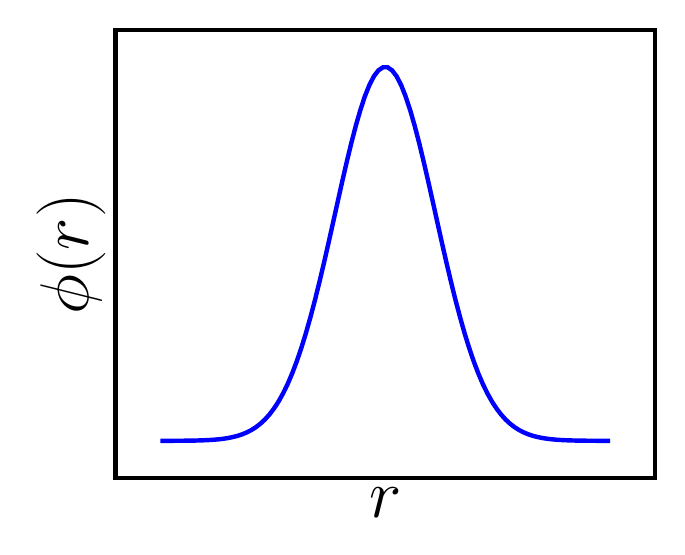
\begin{tikzpicture}
              \begin{axis}[ticks=none,samples=100,ylabel={\Huge $\phi(r)$},xlabel={\Huge $r$}, xlabel near ticks, ylabel near ticks, axis line style=ultra thick]
                \addplot[blue, ultra thick, domain=-1:1] {exp(-x^2*10)};
              \end{axis}
            \end{tikzpicture}
          }
        }
        \only<4,5>{\includesvg[width=\linewidth]{gfx/ibm_interp}}%
      \end{figure}
    }
    \only<3>{\centering Example: $\phi(r) \propto e^{-\frac{r^2}{2\sigma^2}}$}
    \end{column}
  \end{columns}
  \setbeamercovered{transparent=0}
  \onslide<2>{{\footnotesize Supervector notation $\vec{F} := \{\vec{F}_1,\dots,\vec{F}_N\}$}}
\end{frame}

\begin{frame}
  \frametitle{Particle-grid coupling}
  \framesubtitle{GPU thread geometry}
  \includesvg[width=0.8\linewidth]{gfx/cudablocks}\\
  \onslide<2->{
    \centering
    \Large Special considerations:
    \begin{itemize}
    \item<2-> Massively parallel
    \item<3-> Single Instruction Multiple Data (SIMD)
    \item<4-> Mostly memory-bandwidth bound
    \end{itemize}
  }
\end{frame}

\begin{frame}
  \frametitle{Particle-grid coupling}
  \framesubtitle{GPU-friendly algorithm}
  \begin{columns}
    \begin{column}{0.6\linewidth}
      \begin{itemize}
      \item {\color{ForestGreen} $b_i$}: Block assigned to particle $i$.
      \item {\color{red} $t_j$}: Thread $j\in [0:N_b)$ of block $i$, assigned to grid point $n$.
      \end{itemize}
      \begin{block}<2->{\textbf{Spreading:} $\vec{f}_n = \sum_i \vec{F}_i\delta_a(\vec{r}_n-\vec{q}_i)$}
        $t_j\rightarrow$ write to $\vec{f}_n$ \alert<4>{atomically}.
      \end{block}
      \begin{block}<3->{\textbf{Interpolation:} $\vec{u}_i = \sum_n \vec{v}_n\delta_a(\vec{r}_n-\vec{q}_i)h^3$}
        \textbf{1.} $t_j\rightarrow$ gather from $\vec{v}_n$.\\
        \textbf{2.} $t_{\{0\dots 9\}}$ reduce into $\vec{u}_i$.
      \end{block}
    \end{column}
    \begin{column}{0.4\linewidth}
      \includesvg[width=\linewidth]{gfx/ibm_algo}
    \end{column}
  \end{columns}
\end{frame}

\begin{frame}
  \frametitle{Particle-grid coupling}
  \framesubtitle{Performance}
  \centering
  \includegraphics[width=0.6\linewidth]{gfx/ibm_comp_dens1_2080ti}\\
  \begin{minipage}{0.4\linewidth}
    \begin{exampleblock}{Largest number of particles}
      \centering
      $N=512^3 \approx 1.3\cdot 10^8$
    \end{exampleblock} 
  \end{minipage}
  % \begin{columns}[T]
%    \begin{column}{0.4\linewidth}
%    \end{column}
%    \begin{column}{0.6\linewidth}
%
%    \end{column}
%  \end{columns}
\end{frame}

\begin{frame}
  \frametitle{Increasing data locality}
  \only<+>{\includesvg[width=0.8\linewidth]{gfx/celllist0}}%
  \only<+>{\includesvg[width=0.8\linewidth]{gfx/celllist1}}%
  \only<+>{\includesvg[width=0.8\linewidth]{gfx/celllist2}}%
\end{frame}

\begin{frame}
  \frametitle{Particle-grid coupling}
  \framesubtitle{Performance}
  \centering
  \begin{tikzpicture}    
    \begin{scope}
      \draw node[anchor = west, inner sep = 0] (image) {\includegraphics[width=0.49\linewidth]{gfx/ibm_comp_dens1_sorted_2080ti}};
    \end{scope}
    \draw node [above] (text) at (image.north) {\huge Sorted};
    \begin{scope}
      \draw node[anchor = east, inner sep = 0] (image2) {\includegraphics[width=0.49\linewidth]{gfx/ibm_comp_dens1_2080ti}};
    \end{scope}
    \draw node [above] (text2) at (image2.north) {\huge Unsorted};
  \end{tikzpicture}\\
  \begin{minipage}{0.4\linewidth}
    \begin{exampleblock}{Largest number of particles}
      \centering
      $N=512^3 \approx 1.3\cdot 10^8$
    \end{exampleblock}    
  \end{minipage}
\end{frame}

\section{New doubly periodic solvers}
\begin{frame}
  \frametitle{Talk outline}
  \tableofcontents[
  sectionstyle=show/shaded,
  subsectionstyle=show/show/hide,
  subsubsectionstyle=show/show/show/hide
  ]
\end{frame}

\begin{frame}
  \frametitle{Hydrodynamics in confined geometries}
  \framesubtitle{New algorithms for Brownian Dynamics with Hydrodynamic Interactions (BDHI)}
    \begin{figure}
    \centering
    \includesvg[width=0.55\linewidth]{gfx/multiscale}
  \end{figure}  
\end{frame}

\begin{frame}
  \frametitle{Complex fluids}
  \framesubtitle{The spatio-temporal landscape of numerical techniques.}
  \begin{figure}
    \centering    
    \begin{tikzpicture}
      \node[anchor=south west, inner sep=0] (image) {\includesvg[width=0.8\linewidth]{gfx/landscape}};
      \onslide<2>{
        \begin{scope}[shift={(image.south west)},x={(image.south east)},y={(image.north west)}]
        %\draw foreach \xy in {0,0.1,...,1.001}{(\xy,0) -- node[pos=0,below]{\pgfmathprintnumber{\xy}} (\xy,1)(0,\xy) -- node[pos=0,left]{\pgfmathprintnumber{\xy}} (1,\xy)};
%        \only<2>{\filldraw[red, opacity=0.6] (0.12,1) rectangle (0.5,0.07) node[midway] (A) {};\node[above=50pt of A, black]{\contourlength{1pt}\contour{white}{\textbf{Fully Lagrangian}}};}
        \filldraw[blue, opacity=0.6] (0.5,1) rectangle (0.72,0.07) node[midway] (A) {};\node[below=40pt of A, black, align=left]{\contourlength{1pt}\contour{white}{\textbf{Eulerian}}\\\contourlength{1pt}\contour{white}{\textbf{Lagrangian}}};
%        \only<3>{\filldraw[green, opacity=0.6] (0.72,1) rectangle (1,0.07) node[midway] (A) {};\node[above=50pt of A, black]{\contourlength{1pt}\contour{white}{\textbf{Fully Eulerian}}};}
      \end{scope}
      }
    \end{tikzpicture}
    \caption{Figure courtesy of Rafael Delgado-Buscalioni.}
  \end{figure}  
\end{frame}


\subsection{Hydrodynamics}
\begin{frame}
  \frametitle{Smoluchowski level}
  \framesubtitle{Brownian Dynamics with Hydrodynamics Interactions (BDHI)}
  \Large
  \begin{equation*}
    d\vec{\ppos} = \tens{M}\vec{F}dt + \sqrt{2\kT\tens{M}}d\vec{\noise}
    + \kT\vec{\partial}_{\vec{\ppos}}\cdot\tens{M}dt.
  \end{equation*}
  \vspace*{10pt}
  \begin{overlayarea}{\linewidth}{0.6\paperheight}
    \only<1-3>{
      \begin{itemize}
      \item<1-> $\tens{M}(\vec{\ppos})$:\\
        Mobility tensor. Configuration- and BC-dependent
      \item<2-> $d\vec{\noise}$: Brownian motion
      \item<3-> $\kT\vec{\partial}_{\vec{\ppos}}\cdot\tens{M}dt$:\\
        Thermal drift. Zero depending on the BCs
      \end{itemize}
    }
    \only<4->{
      \centering \textbf{Problems}
      \vspace*{10pt}
      \begin{itemize}        
        \setlength\itemsep{10pt}
      \item<5-> $\tens{M}\vec{F}$: Matrix-vector multiplication is $O(N^2)$
      \item<6-> $\sqrt{\tens{M}}$: Quite expensive in general. $O(N^{[2.25-3]})$
      \item<7-> $\tens{M}$ might be unknown/not analytical.
      \end{itemize}
    }
  \end{overlayarea}
\end{frame}
\begin{frame}
  \frametitle{Hydrodynamics}
  %\only<1-4>{\framesubtitle{Incompressible Navier-Stokes equations}}
  %\only<4->{\framesubtitle{Fluctuating Incompressible Navier-Stokes equations}}
  %\only<8->{\framesubtitle{Fluctuating Stokes equations}}
  \framesubtitle{\only<6->{Fluctuating} Stokes equations}
  \begin{equation*}
    \label{eq:navierstokes}
    \begin{aligned}
      %\onslide<1-7>{\overbrace{\underbrace{\rho\partial_t{\vec{\fvel}}}_{\text{time}} +\underbrace{\rho\nabla\cdot (\vec{\fvel}\otimes\vec{\fvel})}_{\text{convection}}}^{\text{fluid inertia}}}
      \onslide<2->{\overbrace{-\eta \nabla^2\vec{\fvel}}^{\text{momentum diffusion}}}
      \onslide<3->{&= \underbrace{-\nabla \pi}_{\text{internal stress}}}
      \onslide<4->{+ \underbrace{\tilde{\vec{f}}}_{\text{\parbox{2cm}{\centering external stress}}}}\\
      \onslide<5->{\nabla\cdot\vec{\fvel} &= 0\quad\mathllap{\underbrace{\phantom{\nabla\cdot\vec{\fvel} = 0}}_{\text{incompressibility}}}}
    \end{aligned}
  \end{equation*}
  \onslide<6->{
    \begin{equation*}
      \tilde{\vec{f}}(\vec{r}) := \underbrace{\vec{f}(\vec{r})}_{\text{external forces}} + \overbrace{\nabla\cdot \mathcal{Z}}^{\text{thermal noise}}
    \end{equation*}
  }
  \onslide<7->{
    \begin{equation*}
      \label{eq:navierstkesnoise}
      \begin{aligned}
        &  \langle \mathcal Z_{ij}\rangle = 0\\
        &  \langle \mathcal Z_{ik}(\vec{\fpos},t)\mathcal Z_{jm}(\vec{\fpos}',t')\rangle = 2\kT\eta(\delta_{ij}\delta_{km} + \delta_{im}\delta_{kj})\delta(\vec{\fpos}-\vec{\fpos}')\delta(t-t')
      \end{aligned}
    \end{equation*}
  }
\end{frame}
\begin{frame}
  \frametitle{Hydrodynamics}
  \framesubtitle{Fluctuating Stokes equations}
  \begin{columns}[T]
    \begin{column}{0.34\linewidth}
      \begin{block}{Stokes equations}
        $%
        \begin{aligned}%
          \nabla \pi - \eta \nabla^2\vec{\fvel} &=  \vec{f} + \nabla\cdot \mathcal{Z}\\
          \nabla\cdot\vec{\fvel} &= 0%
        \end{aligned}
        $%
      \end{block}
      \onslide<2->{
        \begin{minipage}{\linewidth}
          \begin{block}{Fluid forcing}
            \centering $\vec{f}(\vec{r}) = \oper{S}(\vec{r})\vec{F}$
          \end{block}
          \begin{block}{Particle velocity}
            \centering $\vec{u}_i = \oper{J}_{\vec{q}_i}\vec{v}(\vec{r})$
          \end{block}
        \end{minipage}
      }
      \end{column}
      \begin{column}{0.63\linewidth}
        \onslide<3->{
          {
            \begin{center}
              \huge \textbf{Green formalism}
            \end{center}
          }
          \centering $\vec{v} = \oper{G}\tilde{\vec{f}}
          \onslide<4->{
            :=\int{\oper{G}(\vec{r}, \vec{r}^\prime)\tilde{\vec{f}}(\vec{r}) d\vec{r}^\prime}
          }$ %\left(\oper{S}\vec{F} + \nabla\cdot\mathcal{Z}\right)$$
          \onslide<5->{
            \begin{block}{Force Coupling Method (FCM)}
              \centering $\frac{d\vec{q}_i}{dt} = \vec{u}_i = \oper{J}_{\vec{\ppos}_i}\oper{G}(\oper{S}\vec{F} + \nabla\cdot\mathcal Z)$
            \end{block}
          }%
          \begin{overlayarea}{\linewidth}{0.3\paperheight}
            \only<6>{
                \begin{equation*}
                \begin{aligned}
                  &\tens{M} &=&\oper{J}\oper{G}\oper{S}\\
                  &\tens{M}^{1/2} &=&\oper{J}\oper{G}\nabla\cdot\\
                  &\vec{\partial}_{\vec{q}}\cdot\tens{M} &=&0\leftarrow \text{Incompressible}
                \end{aligned}
              \end{equation*}
            }%
            \only<7>{
              \begin{equation*}
                \tens{M}_{ij}=\iint{\delta_a(\vec{r}-\vec{\ppos}_j)\oper{G}(\vec{r},\vec{r}^\prime)\delta_a(\vec{\ppos}_i-\vec{r}^\prime)d\vec{r}^\prime d\vec{r}}
              \end{equation*}
            }%
            \onslide<8->{\centering $\oper{G} :=-\eta^{-1}\nabla^{-2}\left(\mathbb{I} - \nabla\nabla^{-2}\nabla\right)$\\}%
            \onslide<9>{
              \begin{block}{\centering Open boundaries}
                \centering $\oper{G}\rightarrow \tens{O}(\vec{r}) = \frac{1}{8\pi\eta r}\left(\mathbb{I} - \frac{\vec{r}\otimes\vec{r}}{r^2}\right)$
              \end{block}
            }
          \end{overlayarea}
        }
      \end{column}
  \end{columns}
\end{frame}

\begin{frame}
  \frametitle{Hydrodynamics}
  \framesubtitle{Triply periodic FCM}
  \centering
  \huge
  \begin{tikzpicture}[thick]
    \node [style = {draw}] (a) at (0, 4) {$\vec{u}_i= \oper{J}_{\vec{\ppos}_i}\oper{G}(\oper{S}\vec{F} + \nabla\cdot\mathcal Z)$};
    \onslide<2->{
      \node [style = {draw}] (b) at (0, 0) {$\vec{u}_i = \oper{J}_{\vec{\ppos}_i}\onslide<3->{\mathfrak{F}^{-1}}\only<3->{\fou{\oper{G}}}\only<2>{\oper{G}}(\onslide<3->{\mathfrak{F}}\oper{S}\vec{F} + \onslide+<2>{\nabla}\onslide+<3->{\vec{k}}\cdot\mathcal Z)$};
      \draw[->, very thick] (a) to (b);
      \node (c) at (3.2, 2){ $\mathfrak{F}$: Fourier transform};
    }
  \end{tikzpicture}
\end{frame}

\begin{frame}
  \frametitle{Hydrodynamics}
  \framesubtitle{Triply periodic FCM}
  \huge
  $$\vec{u}_i = \oper{J}_{\vec{\ppos}_i}\mathfrak{F}^{-1}\fou{\oper{G}}(\mathfrak{F}\oper{S}\vec{F} + \vec{k}\cdot\mathcal Z)$$
  \begin{block}{\huge\centering Triply Periodic}
    \centering $\fou{\oper{G}}_{\text{3D}} :=\eta^{-1}k^{-2}\left(\mathbb{I} - \frac{\vec{k}\otimes\vec{k}}{k^2}\right)$
  \end{block}
\end{frame}
\begin{frame}
  \frametitle{Hydrodynamics in confined geometries}
  \framesubtitle{New algorithms for Brownian Dynamics with Hydrodynamic Interactions (BDHI)}   
  \begin{columns}[T]
    \begin{column}{0.5\linewidth}
      \begin{itemize}
      \item<1-> Quasi two-dimensional (q2D)
      \item<4-> Doubly periodic (DP)
      \end{itemize}
      \begin{overlayarea}{\linewidth}{0.5\paperheight}
        \only<1-3>{\includesvg[width=0.9\linewidth]{gfx/q2D}\\
          \begin{center}
            q2D: $\delta\rightarrow 0$. 3D fluid, 2D particles
          \end{center}
          }
        \only<4>{\includesvg[width=0.9\linewidth]{gfx/dpstokes_sketch}}
      \end{overlayarea}
    \end{column}
    \begin{column}{0.5\linewidth}
      \begin{overlayarea}{\linewidth}{0.5\paperheight}
        \begin{minipage}{\linewidth}
          \only<2>{
            \begin{block}{Collective diffusion}
              $$D_c(k) \propto H_c(k)$$
              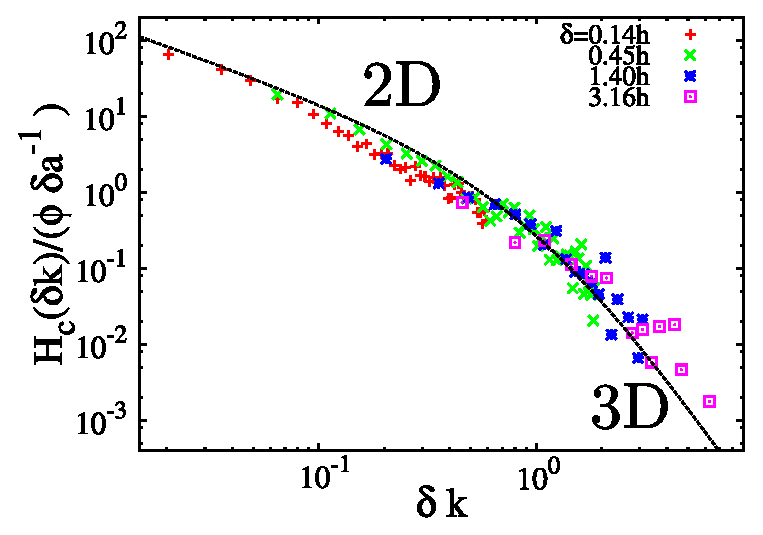
\includegraphics[width=\linewidth]{gfx/q2Dfrom3dto2d}\\
            \end{block}
          }
          \only<3>{\begin{block}{$D_c(k)> 0$ in q2D}          
              \begin{center}
                Correlated density perturbations
                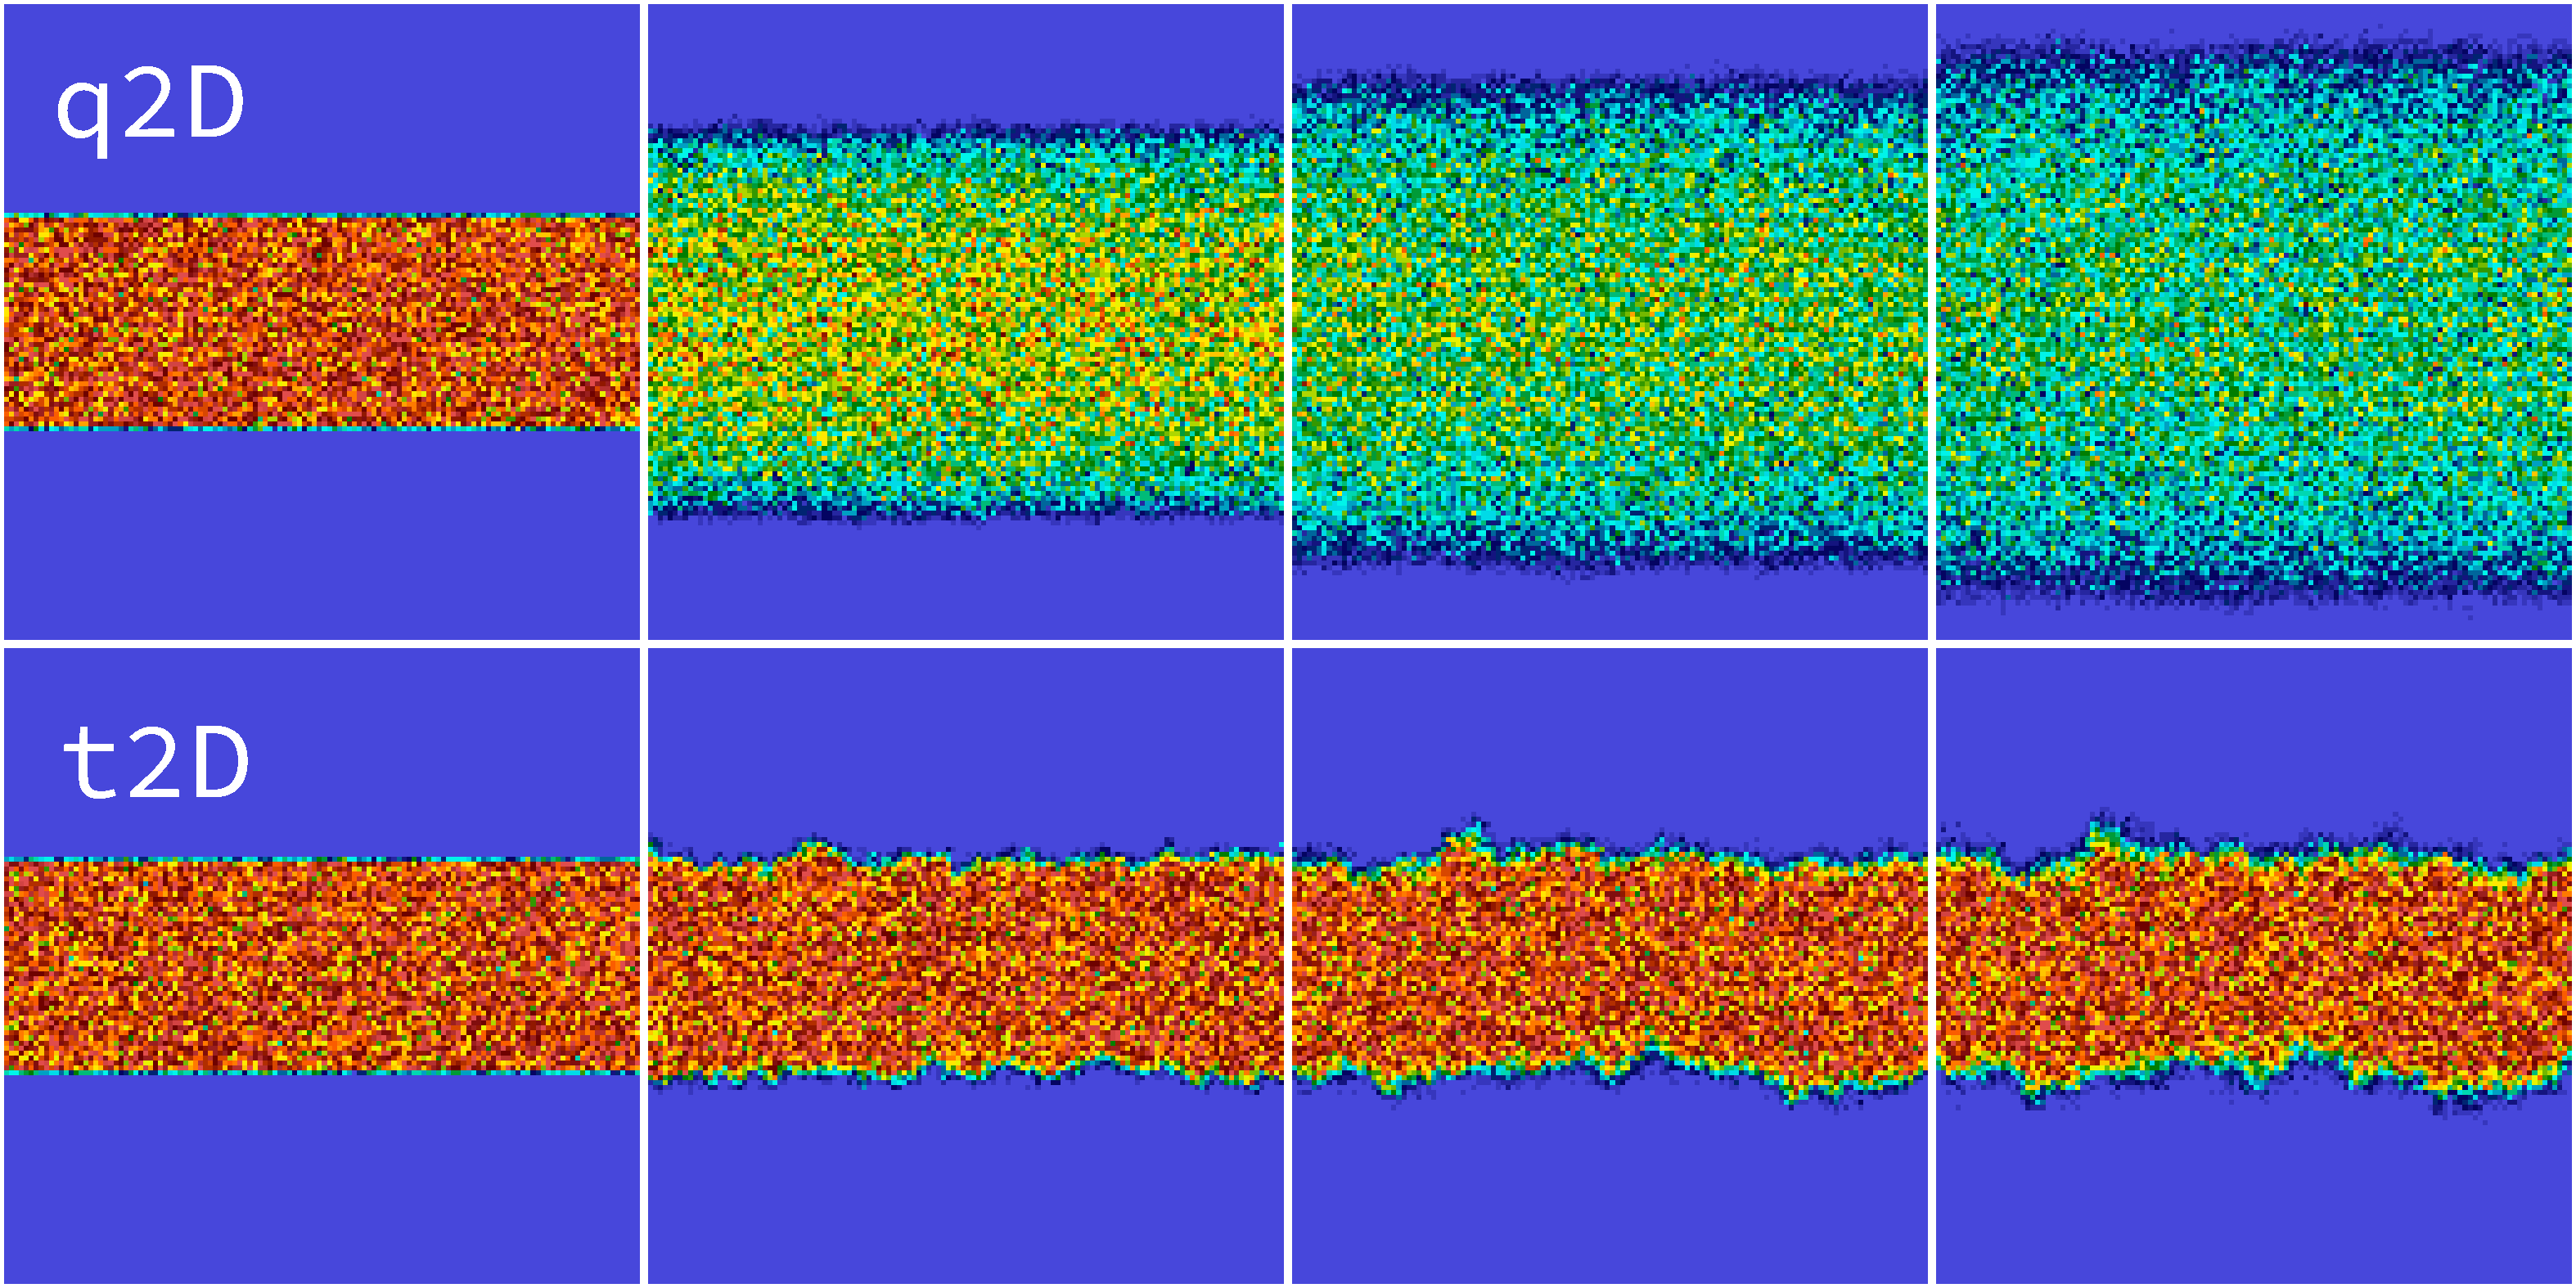
\includegraphics[width=\linewidth]{gfx/q2Dstripes}\\
                \small Time$\rightarrow$
              \end{center}
            t2D: 2D fluid and particles
            \end{block}
          }
        \end{minipage}
      \end{overlayarea}
    \end{column}
  \end{columns}
\end{frame}
\begin{frame}
  \frametitle{Force Coupling Method in quasi 2D}
  \begin{overlayarea}{\linewidth}{0.2\paperheight}
    \begin{block}{\centering Force Coupling Method}
      \begin{center}
        \only<1-7>{$\vec{u}_i = \oper{J}_{\vec{\ppos}_i}\mathfrak{F}^{-1}\fou{\oper{G}}_{\text{3D}}(\mathfrak{F}\oper{S}\vec{F} + \vec{k}\cdot\mathcal Z)$}%
        \only<8-9>{$\vec{u}_i = \oper{J}_{\vec{\ppos}_i}\mathfrak{F}^{-1}\left(\fou{\oper{G}}_{\text{3D}}\mathfrak{F}\oper{S}\vec{F} + \fou{\vec{w}}\right)$}
        \only<10-11>{$\vec{u}_i = \oper{J}_{\vec{\ppos}_i}\mathfrak{F}^{-1}\left(\fou{\oper{G}}_{\qtd}\mathfrak{F}\oper{S}\vec{F} + \fou{\vec{w}}\right)$}
        \only<12->{$\vec{u}_i = \oper{J}_{\vec{\ppos}_i}\mathfrak{F}^{-1}\left(\fou{\oper{G}}_{\qtd}\mathfrak{F}\left[\oper{S}\vec{F} + \vec{\partial}_{\vec{\ppos}}\oper{S}\left(\kT\right)\right] + \fou{\vec{w}}\right)$}
      \end{center}
    \end{block}
  \end{overlayarea}
  \begin{columns}[T]
    \begin{column}{0.4\linewidth}
      \includesvg[width=0.9\linewidth]{gfx/q2D}\\
      \begin{center}
        q2D: $\delta\rightarrow 0$. 3D fluid, 2D particles
      \end{center}
      \onslide<11->{$\vec{\partial}_{\vec{\ppos}}\cdot\left[\oper{J}\oper{G}_{\qtd}\oper{S}\right] \neq 0$}
    \end{column}
    \begin{column}{0.6\linewidth}
      \begin{overlayarea}{\linewidth}{0.7\paperheight}
        \only<1-6>{
          \only<2->{Problems:}
          \begin{enumerate}
          \item<3-> 2D limit implies $F_z\rightarrow \infty$
          \item<4-> Open boundaries in Z require $L_z\rightarrow\infty$ 
          \end{enumerate}
          \only<5->{Solution:}
          \begin{enumerate}
          \item<6> Eliminate Z direction
          \end{enumerate}
        }
        \only<7-12>{
          Eliminate Z direction:
          \begin{enumerate}
          \item<8> Fluctuations via FDT
          \item<9-11> Preconvolve $\oper{G}$ in Z
          \item<12-> Introduce thermal drift
          \end{enumerate}
        }
        \only<8>{
          \begin{center}
            $\left\langle\fou{\vec{w}}\otimes \fou{\vec{w}}\right\rangle = 2\kT \fou{\oper{G}}$
          \end{center}
        }
        \only<9-11>{
          \begin{block}{Remember}
            $\delta_a(\vec{r}) := \phi(r_x)\phi(r_y)\phi(r_z)\rightarrow$ Smeared delta
          \end{block}
        }
        \only<10>{
          \begin{center}
            $\fou{\tens{G}}_{\qtd}(\vec{k}^{\parallel}) = \frac{1}{2\pi}\int\fou{\phi}(k_z)^2\fou{\tens{G}}_{\text{3D}}(\vec{k}^{\parallel},k_z)dk_z$
          \end{center}
        }
        \only<11>{
          \begin{center}
            $\fou{\tens{G}}_{\qtd}(\vec{k}) = \eta^{-1}\left(g(k)\vec{k}^{\perp}\otimes\vec{k}^{\perp} + f(k)\vec{k}\otimes\vec{k}\right)$
          \end{center}
        }
        \only<12>{
          \begin{center}
            $\vec{f}(\vec{r}) = \oper{S}\vec{F} + \vec{\partial}_{\vec{\ppos}}\oper{S}[\kT]$
        \end{center}
        }
      \end{overlayarea}
    \end{column}
  \end{columns}
\end{frame}

\subsection{Electrostatics}
\begin{frame}
  \frametitle{Triply Periodic Electrostatics}
  \framesubtitle{Force Coupling Method for the Poisson equation}
  \begin{center}
    \begin{minipage}{0.5\linewidth}    
      \begin{block}{Poisson}
        \centering $\varepsilon\nabla^2\phi = -f(\vec{r}) = -\oper{S}(\vec{r})\vec{Q}$
      \end{block}
    \end{minipage}
  \end{center}
  \begin{overlayarea}{\linewidth}{0.5\paperheight}
    \begin{columns}[T]
      \begin{column}{0.4\linewidth}
        \begin{block}<2->{Spreading}
          $\oper{S}(\vec{r})\vec{Q} = \sum_i Q_i \delta_a(\vec{\ppos}_i - \vec{r})$
        \end{block}
        \begin{block}<3->{Gaussian sources}
          $\delta_a(\vec{r}) = \frac{1}{(2\pi a^2)^{3/2}} e^{-r^2/(2a^2)}$
        \end{block}
        
      \end{column}
      \begin{column}{0.6\linewidth}
        \begin{block}<4->{Charges to forces}
          $$\vec{F}_i = Q_i\oper{J}_{\vec{q}_i}\mathfrak{F}^{-1}i\vec{k}\fou{\oper{G}}_P\mathfrak{F}\oper{S}\vec{Q}$$
        \end{block}
        \only<4->{$$\fou{\oper{G}}_P = \varepsilon^{-1}k^{-2}$$}
        
      \end{column}
    \end{columns}
  \end{overlayarea}
  \only<1-3>{\footnotesize Supervector notation. Charges $\vec{Q} := \{\vec{Q}_1,\dots,\vec{Q}_N\}$}
\end{frame}
%\section{Introduction}
%\begin{frame}
%  \frametitle{\insertsection}
%  \begin{itemize}
%  \item Outline
%  \item Physics, algorithms and implementation
%  \item This thesis contributions
%  \end{itemize}
%\end{frame}
%
%\subsection{Complex fluids}
%\begin{frame}
%  \frametitle{\insertsubsectionnavigation{\linewidth}}
%  \begin{itemize}
%  \item What a complex fluid is and why we care
%  \item Coarse-graining
%  \end{itemize}
%\end{frame}
%\subsubsection{A typical system of interest}
%\begin{frame}
%  \frametitle{\insertsubsectionnavigation{\linewidth}} 
%  \framesubtitle{\insertsubsubsection}
%  \begin{itemize}
%  \item ``We want to study this particular system (a virus?, QCM?)''
%  \item Problems that arise when trying to simulate this system
%  \item The message is: We need new theory and algorithms. If we carefully design a software for a system like this, we end up with something that is also valid for things like MD,  SPH, DPD,...
%  \end{itemize}
%\end{frame}
%\subsection{High performance computing in complex fluids}
%\begin{frame}
%  \frametitle{\insertsubsectionnavigation{\linewidth}} 
%  \begin{itemize}
%  \item The GPU
%  \item Other software packages
%  \item Trying to keep it simple
%  \end{itemize}
%\end{frame}
%
%
%\section{The different ingredients of a complex fluid simulation}
%
%\begin{frame}
%  \frametitle{\insertsectionnavigation{\linewidth}} 
%  \begin{itemize}
%  \item Hydrodynamics
%  \item Particle interactions
%  \item Electrostatics
%  \end{itemize}
%\end{frame}
%
%\subsection{Hydrodynamics}
%\begin{frame}
%  \frametitle{\insertsubsectionnavigation{\linewidth}}
%  \begin{itemize}
%  \item Fluid dynamics
%  \item Particle-fluid coupling (IBM)
%  \item Pseudo-spectral solvers (FCM)
%  \end{itemize}
%\end{frame}
%
%\subsection{Particle interactions}
%\begin{frame}
%  \frametitle{\insertsubsectionnavigation{\linewidth}}
%  \begin{itemize}
%  \item Neighbour lists
%  \item bonds
%  \end{itemize}
%\end{frame}
%
%\subsection{Electrostatics}
%\begin{frame}
%  \frametitle{\insertsubsectionnavigation{\linewidth}}
%  \begin{itemize}
%  \item Poisson equation
%  \item Reuse of FCM
%  \end{itemize}  
%\end{frame}
%    
%\subsection{UAMMD: A GPU framework for complex fluids}
%\begin{frame}
%  \frametitle{\insertsubsectionnavigation{\linewidth}} 
%  \begin{itemize}
%  \item What UAMMD is and tries to achieve
%  \item ``UAMMD has enabled the community to study hydrodynamics in new systems''
%  \item Not trying to sell UAMMD, just showcase what it can do.    
%  \end{itemize}
%\end{frame}
%
%\section{New physics}
%
%\begin{frame}
%  \frametitle{\insertsectionnavigation{\linewidth}} 
%  \begin{itemize}
%  \item List works using UAMMD, what level of detail here?
%  \end{itemize}
%\end{frame}
%

\section{UAMMD}
\begin{frame}
  \frametitle{Talk outline}
  \tableofcontents[
  sectionstyle=show/shaded,
  subsectionstyle=show/show/hide,
  subsubsectionstyle=show/show/show/hide
  ]
\end{frame}

\begin{frame}
  \frametitle{The sea of packages}
  \includesvg[width=\linewidth]{gfx/mdpacks}
\end{frame}

\begin{frame}
  \frametitle{What makes UAMMD stand out}
  
  \begin{itemize}
    \Large
  \item Header only and library-like
  \item Lightweight with minimal dependencies
  \item Hackable
  \item Focus on hydrodynamics
  \end{itemize}
\end{frame}

\subsection{Universally Adaptable Multiscale Molecular Dynamics}
\begin{frame}[t]
  \frametitle{UAMMD}
  \framesubtitle{Universally Adaptable Multiscale Molecular Dynamics}
  \begin{overprint}
    \onslide<+>
    \centering \huge \bf Universal
    \onslide<+>
    \centering \huge \bf Adaptable
    \onslide<+>
    \centering \huge \bf Multiscale
    \onslide<+>
    \centering \huge \bf Molecular Dynamics
  \end{overprint}
  \begin{columns}[T]
    \begin{column}{0.65\linewidth}
      \begin{overlayarea}{\linewidth}{0.6\paperheight}
        \begin{figure}
          \only<1>{%
            \includesvg[width=0.9\linewidth]{gfx/universally}%
          }%
          \only<2>{%
            \includesvg[width=0.8\linewidth]{gfx/virus}%
          }%
          \only<3>{%
            \includesvg[width=0.8\linewidth]{gfx/scales}%
          }%
          \only<4>{%
            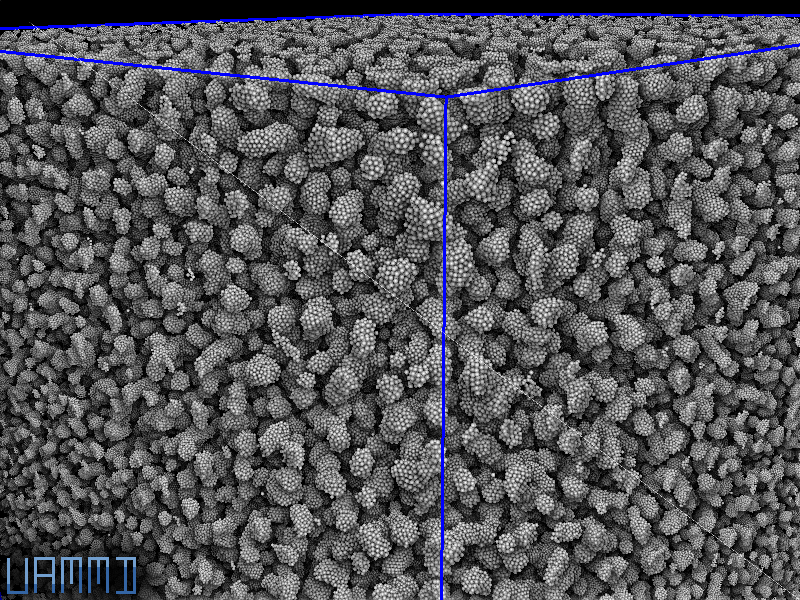
\includegraphics[width=0.9\linewidth]{shotlogo}%
          }%
        \end{figure}
      \end{overlayarea}
    \end{column}
    \begin{column}{0.35\linewidth}      
      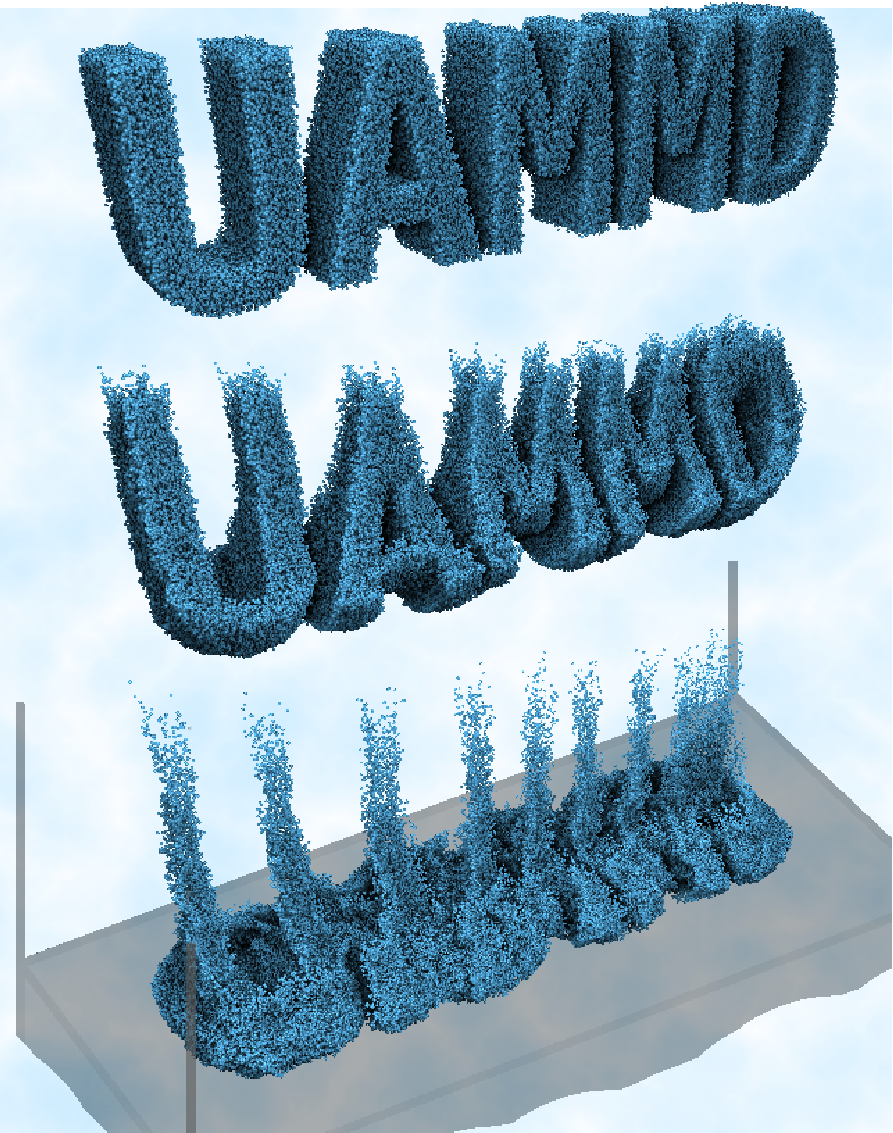
\includegraphics[width=1.0\linewidth]{poster.png}
     \end{column}
   \end{columns}
   \only<1>{\Large Lagrangian and Eulerian descriptions.}%
   \only<2>{\Large Independent building blocks.}%
   \only<3>{\Large Solvers for many scales.}%
   \only<4>{\Large Mainly particle based.}%
\end{frame}
\subsection{Basic code structure}
\begin{frame}[fragile]
  \frametitle{UAMMD}
  \framesubtitle{Conceptual hierarchy}
  \includesvg[width=\linewidth]{gfx/sketchUAMMD}
  \begin{overprint}
    \onslide<2>
    \begin{code2}[]{label=code:module}
      #include<uammd.cuh>
      int main(int argc, char* argv[]){
        auto sys = std::make_shared<System>(argc, argv);
        ...
    \end{code2}
    \onslide<3>
    \begin{code2}[]{label=code:module}
      #include<uammd.cuh>
      int main(int argc, char* argv[]){
        auto sys = std::make_shared<System>(argc, argv);
        const int nP = 1e6; //Number of particles
        auto pd = std::make_shared<ParticleData>(nP, sys);
        ...
      \end{code2}
      \onslide<4>
    \begin{code2}[]{label=code:module}
      ...
      auto pos = pd->getPos(access::cpu, access::write);
      pos[0] = {1,1,1,0}; // x,y,x, color (type)
      ...
    \end{code2}
    \onslide<5>
    \begin{code2}[]{label=code:module}
      ...
      auto md = std::make_shared<VerletNVE>(pd, /*Parameters*/);
      md->forwardTime(); //Exposed by every Integrator
      ...      
    \end{code2}
    \onslide<6>
    \begin{code2}[]{label=code:module}
      ...
      auto electro = std::make_shared<Poisson>(pd,
                                              /*Parameters*/);
      //Exposed by every Integrator
      md->addInteractor(electro); 
      md->forwardTime();
      ...      
    \end{code2}
  \end{overprint}
\end{frame}
  
\begin{frame}
  \frametitle{Available solvers}
    \includesvg[width=\linewidth]{gfx/sketchUAMMD_integrators}
\end{frame}

\begin{frame}
  \frametitle{Available interactions}
  \includesvg[width=\linewidth]{gfx/sketchUAMMD_interactors}
  \note{We are already generalizing. Talk about the new interactions people are including: Optohydro, magnetism, coarse-grained potentials...}
\end{frame}

\section{Conclusions}
\begin{frame}
  \setbeamercovered{transparent=40}
%  \setbeamertemplate{itemize/enumerate subbody begin}{\vspace{0.5cm}}
  \setbeamertemplate{itemize/enumerate subbody end}{\vspace{1cm}}
  \frametitle{This thesis main contributions}
  \begin{enumerate}
    \Large\color{blue}
  \item \textbf{Software}.
    \begin{itemize}
    \item<+-> UAMMD: Complex fluids in the GPU      
    \item<+-> Superpunto: A particle visualizator
    \item<+-> GPU post-processing tools: RDF, MSD, correlations...
    \end{itemize}
  \item<+-> \textbf{Algorithms}.
    \begin{itemize}
    \item<+-> Electrostatics and Hydrodynamics in doubly periodic domains.
    \item<+-> Eulerian-Lagrangian coupling.
    \end{itemize}
  \item<+-> \textbf{Physics}.
    \begin{itemize}
    \item<+-> Colloid diffusion under soft (and hard) two-dimensional confinement.
    \item<+-> Dynamics of star-polymer solutions.
    \item<+-> Intra-cellular viscosity.
    \end{itemize}
%  \item Use this slide to give an outline of the talk
  \end{enumerate}
\end{frame}

\end{document}